\documentclass[a4j]{jarticle}
\usepackage[dvipdfmx]{graphicx}
\usepackage{amssymb}
\usepackage{subfigure}
\usepackage{longtable}

\begin{document}
\begin{table}[t]
\begin{center}
{\large 産業用モニタリングシステムにおける障害検知手法の提案}\\
令和 2 年 7 月 20 日\\
山本 航平
\end{center}
\end{table}

進捗報告
\begin{itemize}
\item グローバル IP アドレスの範囲を調べました
\item 10 ミリ秒間隔での計測を行いました
\item 計測中に(一時間毎に)グローバルIPアドレスを取得し始めました.以前メールにてご報告させていただいた「210.138.0.0/16」「210.149.0.0/16」に加えて「203.180.0/0/16」が確認できました.
\end{itemize}

\section{10 ミリ秒間隔での計測}
ping による応答遅延の計測を 10 ミリ秒間隔で計 10 回行う操作を 5 秒毎に実行したところ,図 \ref{short} のような右下がりの傾向が見れらている.この図では,ping コマンドの実行時刻が早いものから順に $t = 1,2,\ldots$ とし,$t$ を横軸に,縦軸にはそれに対応する ping 応答遅延時間 [ms] をとり,縦軸に垂直な黒線で ping の実行時刻に応じた組分けて組内の ping の実行間隔は 10 ミリ秒,組間の先頭の ping の実行間隔が 5 秒となるようにしている.
\begin{figure}[tb]
\begin{center}
\subfigure[$0 \sim 1$ 分後]{
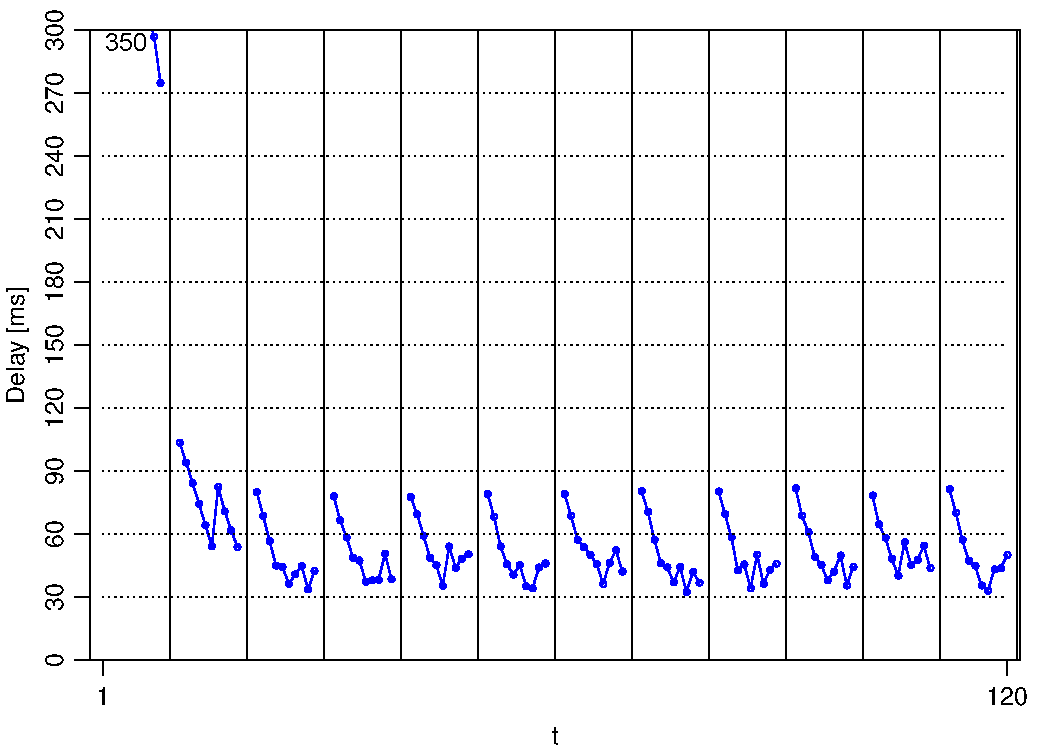
\includegraphics[width=0.33\hsize]{../2020-07-02/0-1.pdf}
}~
\subfigure[$1 \sim 2$ 分後]{
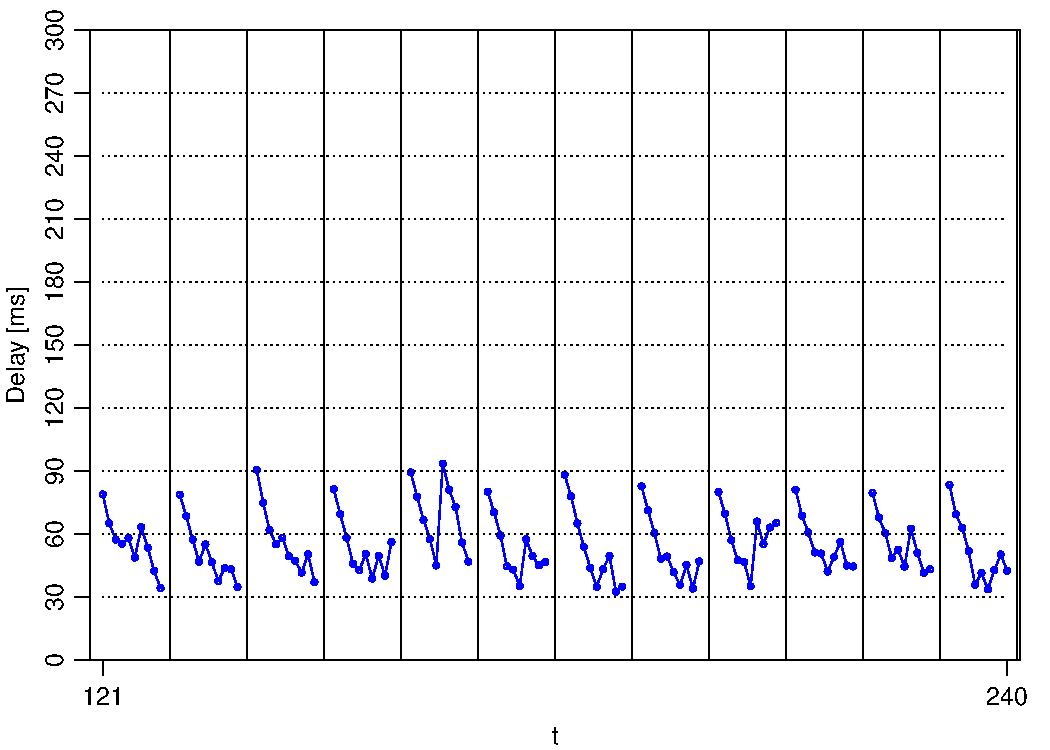
\includegraphics[width=0.33\hsize]{../2020-07-02/1-2.pdf}
}~
\subfigure[$2 \sim 3$ 分後]{
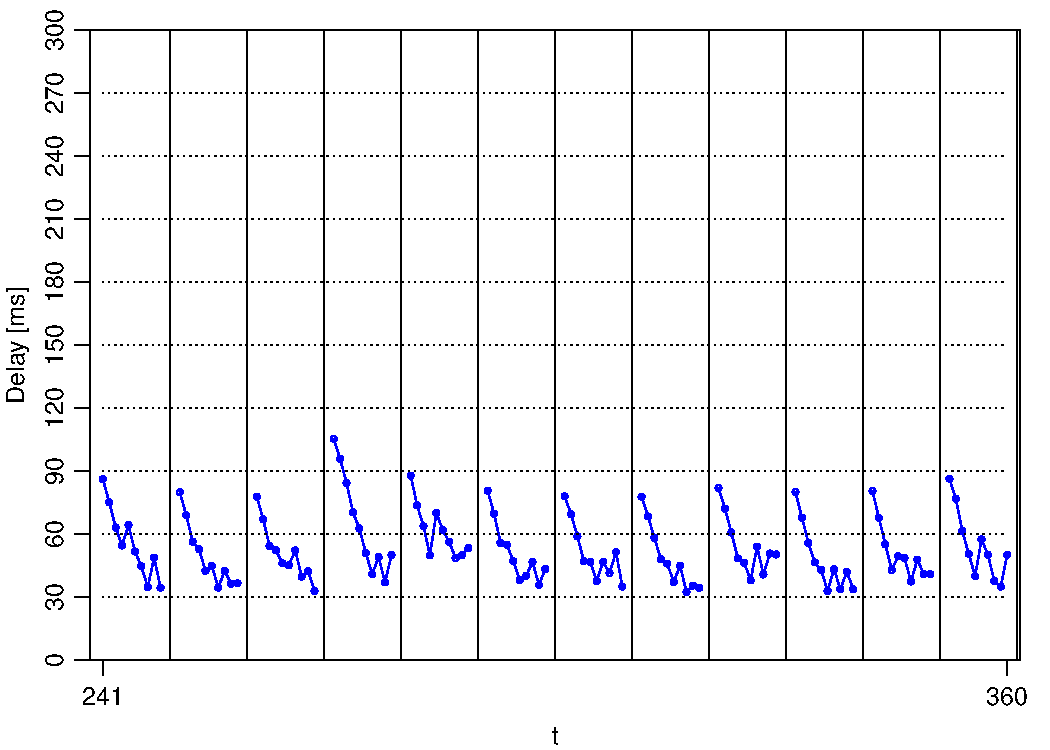
\includegraphics[width=0.33\hsize]{../2020-07-02/2-3.pdf}
}
\caption{10 ミリ秒間隔で計 10 回の ping 実行を 5 秒毎に行った計測結果(一部抜粋)}
\label{short}
\end{center}
\end{figure}

この計測では 10 ミリ秒間隔で計 10 回の 100 ミリ秒間でしか右下がりの傾向を捉えておらず,その後は小さな応答遅延で安定するのか,もしくはどこかのタイミングで増加し右下がりの変化が再度見られるのかがわからない.
そこで,計測時間延ばして 20 分間行い 100 ミリ秒後の変化の仕方を調べた.その結果を図 \ref{long} に示す.この図は,ping コマンドの実行時刻が早いものから順に $t = 1,2,\ldots,120000$ とし,$t$ を横軸に,縦軸にはそれに対応する ping 応答遅延時間 [ms] をとったものであり,図 \ref{long1} は計測開始から 1 秒後まで,図 \ref{long2} は計測開始から 1 分後まで,図 \ref{long3} は計測開始から 20 分後までを示している.
\begin{figure}[tb]
\begin{center}
\subfigure[計測開始から 1 秒後まで]{
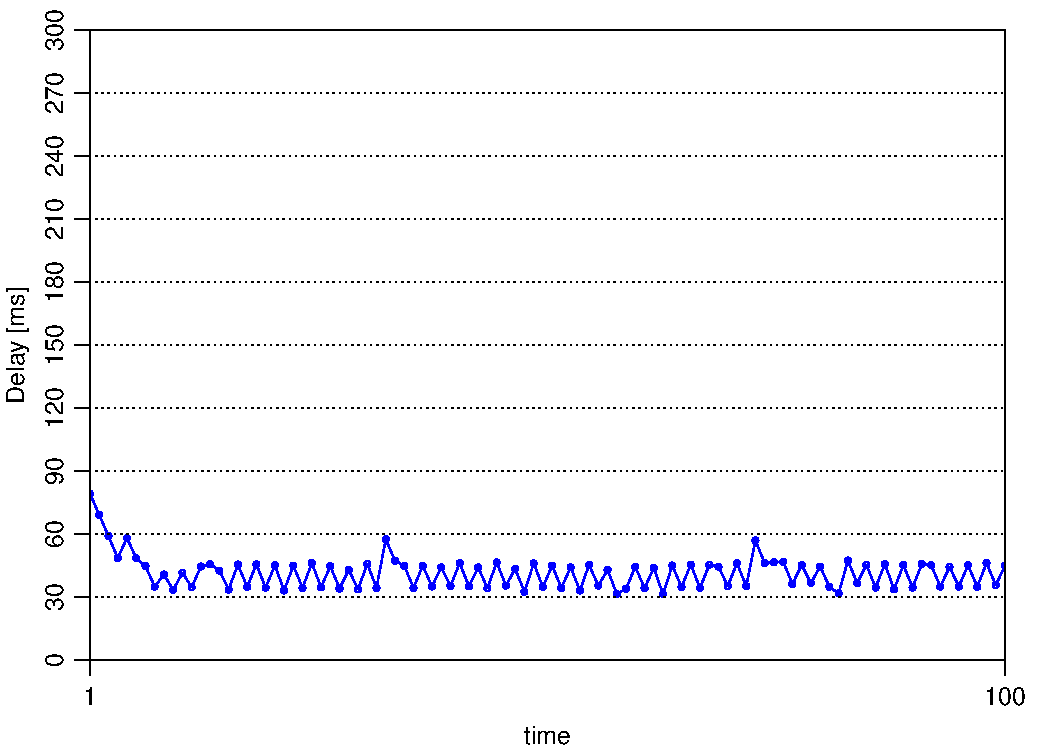
\includegraphics[width=0.5\hsize]{../2020-07-20/1-100.pdf}
\label{long1}
}\\
\subfigure[計測開始から 1 分後まで]{
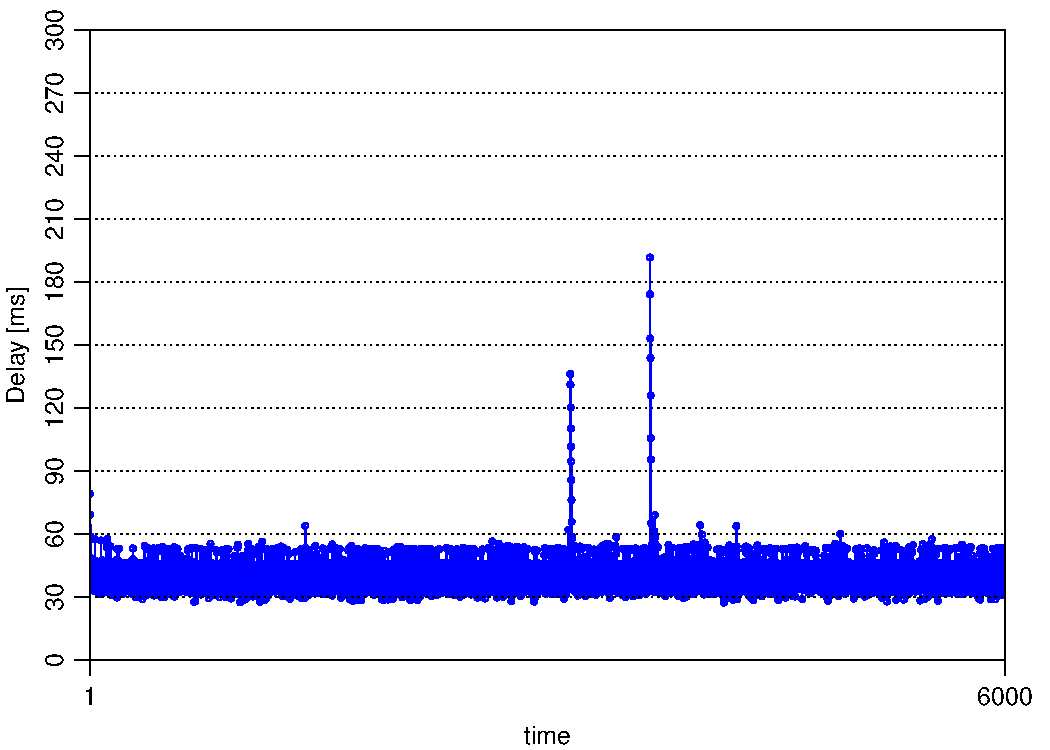
\includegraphics[width=0.5\hsize]{../2020-07-20/1-6000.pdf}
\label{long2}
}~
%\subfigure[計測開始から 20 分後まで]{
%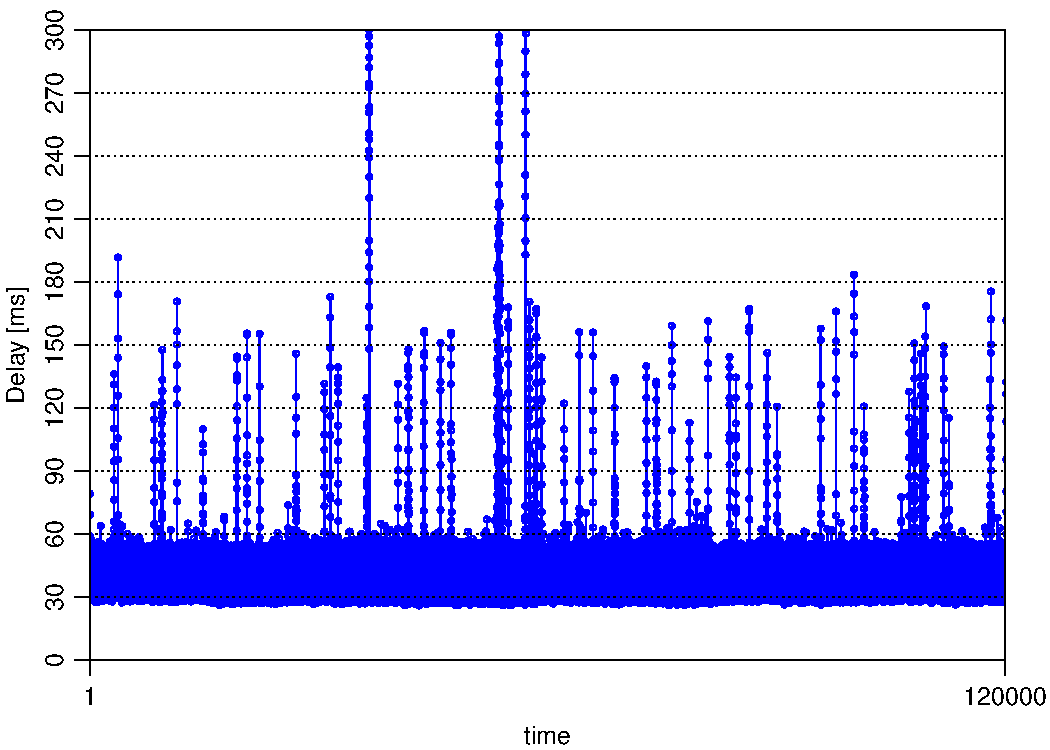
\includegraphics[width=0.5\hsize]{../2020-07-20/1-120000.pdf}
%\label{long3}
%}
\caption{10 ミリ秒間隔で 20 分間の ping 応答遅延計測}
\label{long}
\end{center}
\end{figure}
図\ref{long1} より,計測開始直後は図 \ref{short} と同様の右下がりの応答遅延の減少が見て取れ,約 30 ミリ秒まで減少するとその後はおおよそ 30 ミリ秒から 40 ミリ秒までの小さな値の範囲で変化していた.なお,ping の宛先を同じ AWS サーバとし 15 秒間隔で計測を行うと,応答遅延は図 \ref{6-23} のように 60 ミリ秒以上の値を取る.
\begin{figure}[tb]
\centering
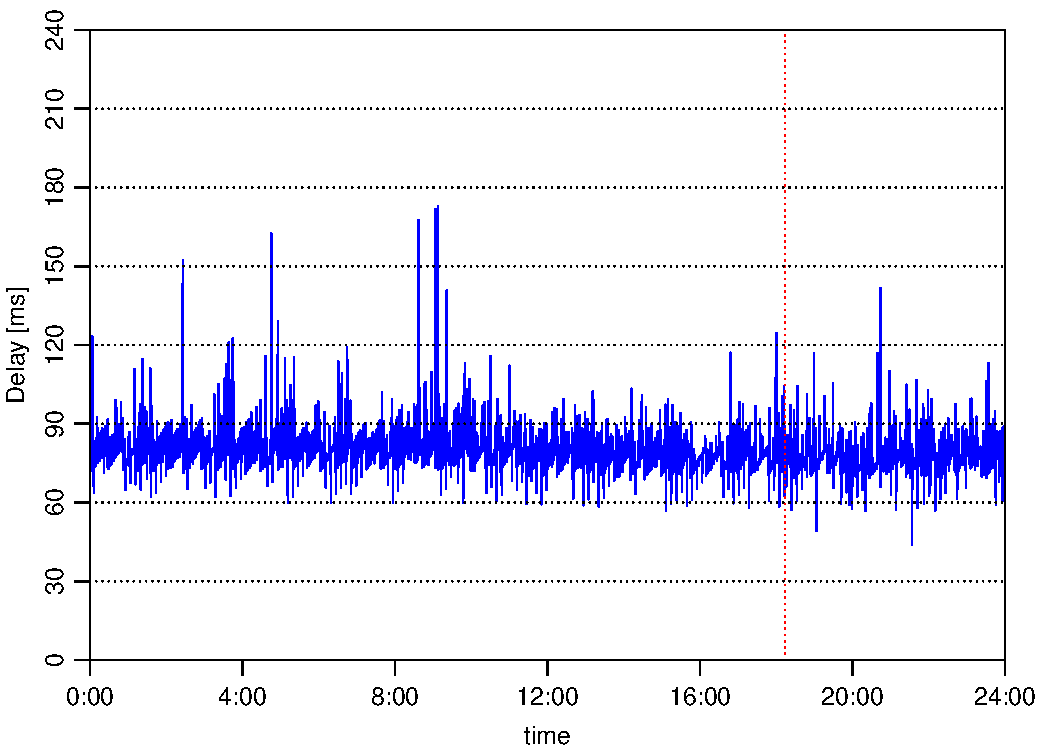
\includegraphics[width=0.8\hsize]{../2020-07-08/plot-6-23.pdf}
\caption{15 秒間隔での計測(6 月 23 日)}
\label{6-23}
\end{figure}
一方,図 \ref{long2} や図 \ref{long3} では 120 ミリ秒を超える大きな応答遅延が計測された.このことから,ping の実行間隔を 10 ミリ秒と短くすることで作られる連続的な通信状況では,計測始めは少し大きな応答遅延時間が計測されるが,その後は減少していきやがて 30 ミリ秒程度の伝搬遅延時間を考慮した最小応答遅延時間まで達し,以降はその近傍の小さな値を推移するが,時折 100 ミリ秒程度の時間幅で 120 ミリを超える大きな応答遅延が発生することが分かった.

また,図 \ref{long3} では 90 ミリ前後の応答遅延が複数回計測されており,この値は図 \ref{6-23} に示した 15 秒間隔での計測で主に確認されている応答遅延時間である.そのため,図 \ref{6-23} の 15 秒間隔での計測結果は図 \ref{long3} の 10 ミリ秒間隔での計測結果を 15 秒毎に抽出したものではないかと考えた.図 \ref{ext} は図 \ref{long3} から 15 秒間隔で応答遅延を抜き出したものである.
\begin{figure}
\centering
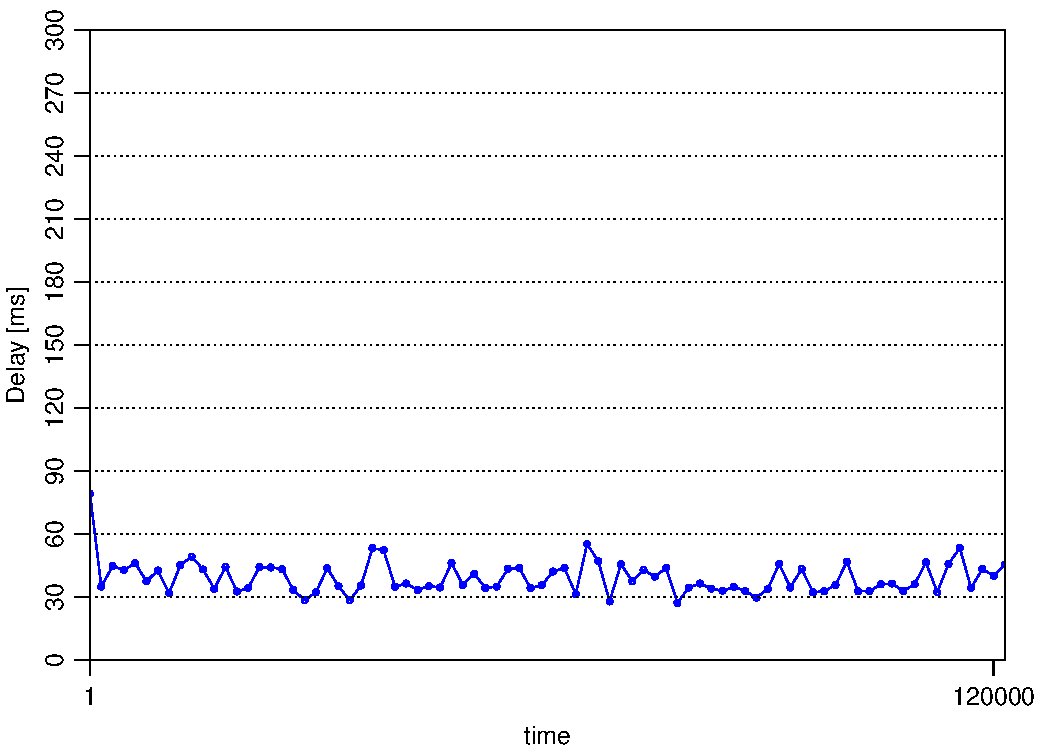
\includegraphics[width=0.8\hsize]{../2020-07-20/ext.pdf}
\caption{\ref{long3} から 15 秒毎の応答遅延時間を抽出}
\label{ext}
\end{figure}
図 \ref{ext} が図 \ref{6-23} と似通った波形となることを期待したのだが,明らかに図 \ref{ext} での応答遅延時間は小さな値で変動も小さいものとなっていた.これは 10 ミリ秒間隔での計測で得られる 90 ミリ秒程度の応答遅延はごく少数であり,その他のほとんどが 30 ミリ秒から 60 ミリ秒までの小さな応答遅延帯に分布しているからだと考えられる.図 \ref{5ms} は図 \ref{long3} で示された 10 ミリ間隔で 20 分間行った計測の応答遅延の分布であり,図 \ref{15s} は図 \ref{6-23} で示された 15 秒間隔で 24 時間行った計測の応答遅延分布である.また,これらの図は正規化しており,ビン幅は 1 ミリ秒である.
\begin{figure}[tb]
\begin{center}
\subfigure[10 ミリ秒間隔の計測に対して]{
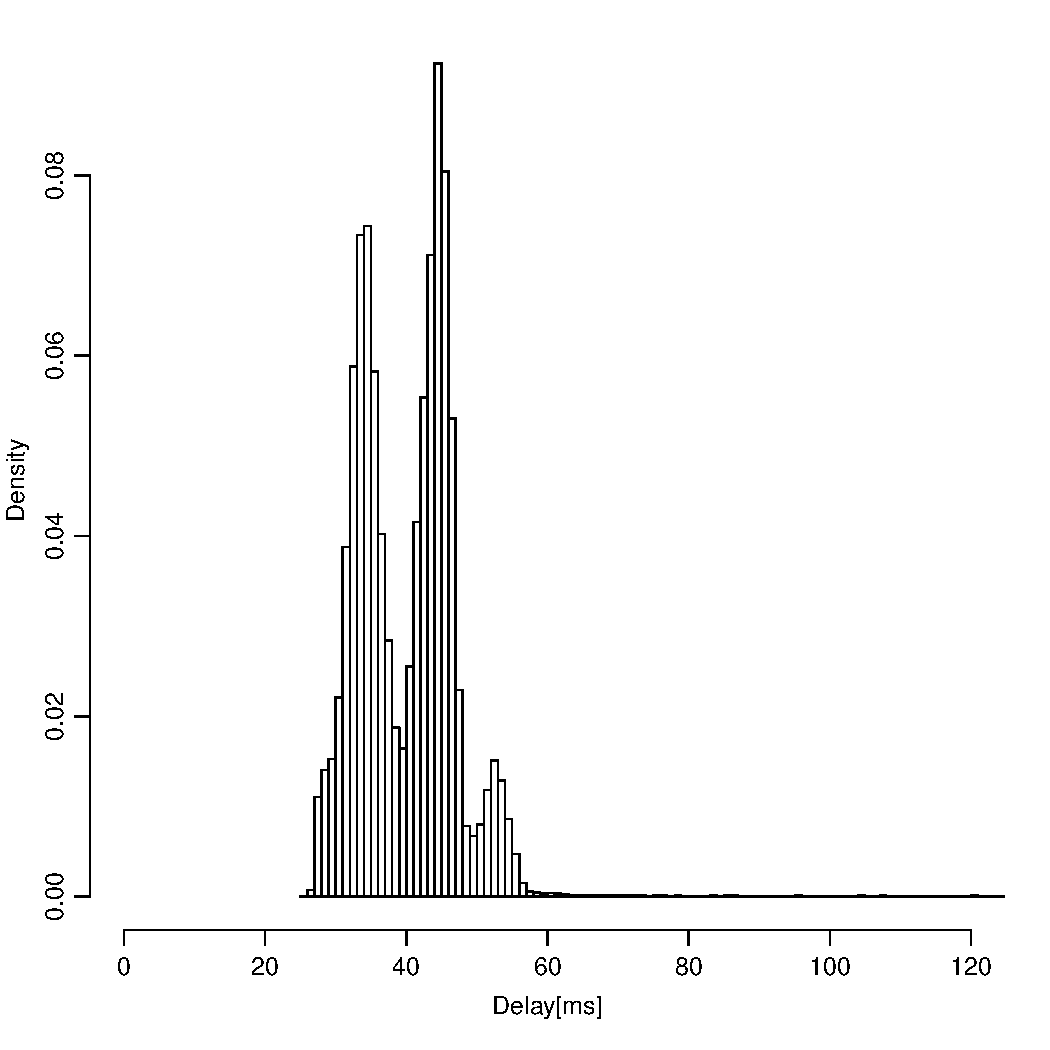
\includegraphics[width=0.5\hsize]{../2020-07-20/5s-hist.pdf}
\label{5ms}
}~
\subfigure[15 秒間隔の計測に対して]{
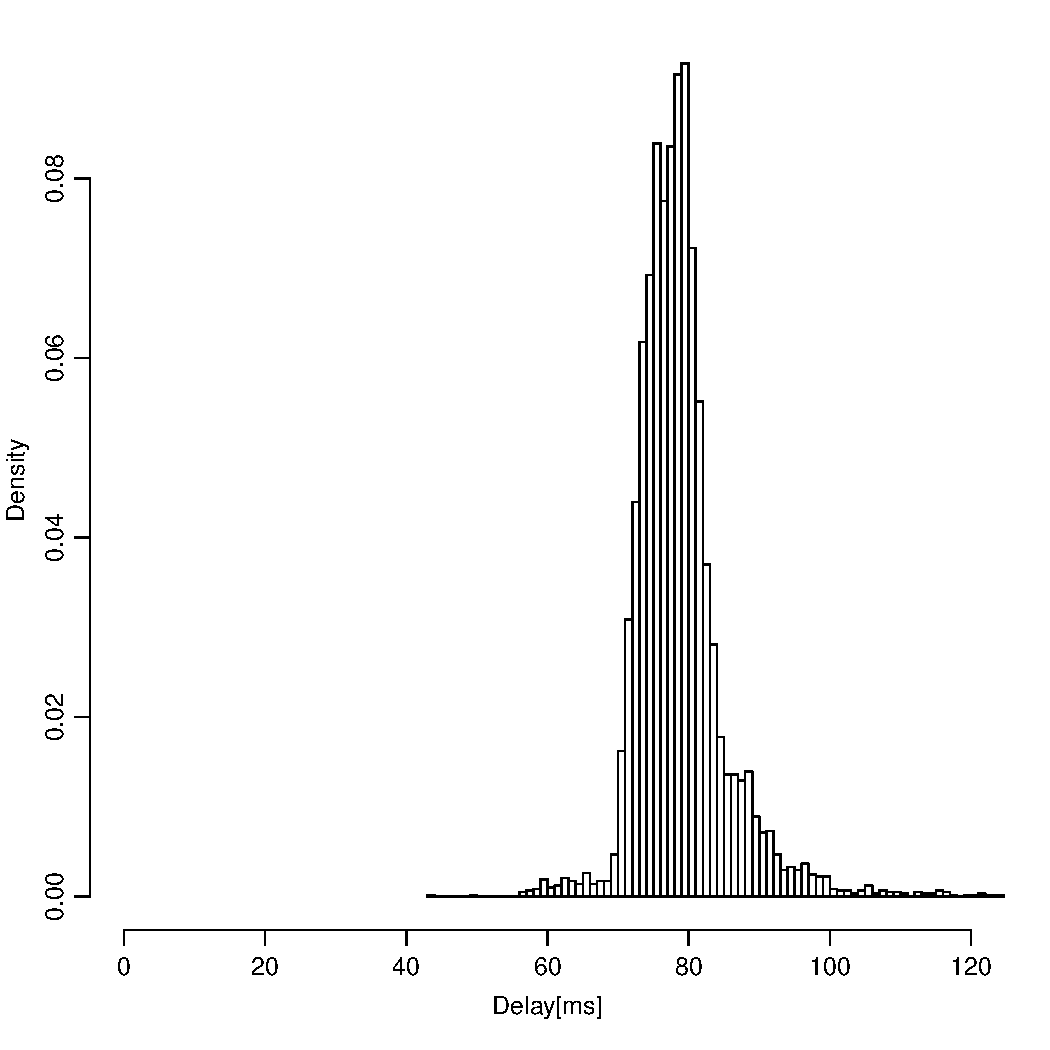
\includegraphics[width=0.5\hsize]{../2020-07-20/15s-hist.pdf}
\label{15s}
}
\caption{応答遅延分布}
\end{center}
\end{figure}
\end{document}